\documentclass[aspectratio=169, table, 12pt]{beamer}

\usepackage{colortbl}
\usepackage{xcolor}
\usepackage{listings}
\usepackage{tabularx}
\usepackage{tikz}
\usetikzlibrary{arrows.meta, positioning, calc, fit, shapes.geometric}

\makeatletter
\def\input@path{{../theme/}}
\makeatother
\graphicspath{{../theme/}{../../figures/}}
\usetheme{Pradita}

\definecolor{praditagreen}{RGB}{37, 113, 71}

% Tema membuat garis tabel berwarna putih. Dikembalikan agar tabel terbaca.
\arrayrulecolor{black}
\setlength{\arrayrulewidth}{0.5pt}

% Menempatkan gambar di tengah kolom, mendatar sekaligus tegak. Lebarnya
% dipenuhi selebar kolom. Bila hasilnya melebihi tinggi yang disediakan,
% tingginya yang menjadi pembatas, sehingga gambar tidak menembus bingkai.
\newsavebox{\kotakkolom}
\newcommand{\gambarkolom}[2][0.72\textheight]{%
  \sbox{\kotakkolom}{\resizebox{\linewidth}{!}{#2}}%
  \begin{minipage}[c][#1][c]{\linewidth}%
    \centering
    \ifdim\dimexpr\ht\kotakkolom+\dp\kotakkolom\relax>#1\relax
      \resizebox{!}{#1}{#2}%
    \else
      \usebox{\kotakkolom}%
    \fi
  \end{minipage}%
}

\lstdefinestyle{PythonStyle}{
  language=Python,
  basicstyle=\ttfamily\scriptsize,
  keywordstyle=\color{blue}\bfseries,
  commentstyle=\color{gray}\itshape,
  stringstyle=\color{red},
  breaklines=true,
  frame=lines,
  backgroundcolor=\color{lightgray!10},
  tabsize=2,
  showstringspaces=false
}

\lstdefinelanguage{bash}{
  keywords={},
  basicstyle=\ttfamily\scriptsize,
  ndkeywords={cd, python, bash, source},
  ndkeywordstyle=\color{purple}\bfseries,
  sensitive=true,
  commentstyle=\color{gray},
  breaklines=true,
  frame=lines,
  backgroundcolor=\color{lightgray!10},
  tabsize=2,
  comment=[l]{\#},
  showstringspaces=false
}

\title{\Huge{Pipeline/\\Pipe-and-Filter}}
\subtitle{IF231303 Arsitektur Perangkat Lunak}
\author{Alfa Yohannis}

\begin{document}

\frame{\titlepage}

\begin{frame}{{\Large Tujuan Pembelajaran}}
  \vspace{10pt}
  \begin{enumerate}
    \item Menjelaskan pembagian antara \textit{filter} dan \textit{pipe} beserta
          \textit{contract} yang menyambung keduanya.
    \item Membedakan pemrosesan \textit{streaming} dari pemrosesan
          \textit{batch}, lalu menentukan kapan masing-masing layak dipilih.
    \item Mengukur \textit{filter independence}, akibat \textit{stage
          reordering}, dan \textit{first output latency}.
  \end{enumerate}

  \vspace{10pt}
  {\small Contohnya penyeragaman \textit{file} gambar, yaitu foto dari sumber
  beragam diubah menjadi beberapa resolusi baku bertanda air.}
\end{frame}

\begin{frame}{{\Large Pendahuluan}}
  \vspace{8pt}
  \begin{itemize}\small
    \item Pekerjaan ditata menjadi deretan \textit{stage}, tiap \textit{stage}
          mengerjakan satu perubahan kecil.
    \item \textit{Stage}-nya disebut \textit{filter}, penyambungnya disebut
          \textit{pipe}, dan rangkaiannya disebut \textit{pipeline}.
  \end{itemize}

  \vspace{8pt}
  {\small Pustaka scikit-learn menyediakan kelas \texttt{Pipeline} sendiri,
  dan menuntut setiap \textit{stage} selain yang terakhir memiliki metode
  \texttt{transform}. \textit{Contract} seragam seperti itu yang dipakai pula
  pada contoh bab ini.}
\end{frame}

\begin{frame}{{\Large \textit{Filter} dan \textit{Pipe}}}
  \vspace{14pt}
  \centering
  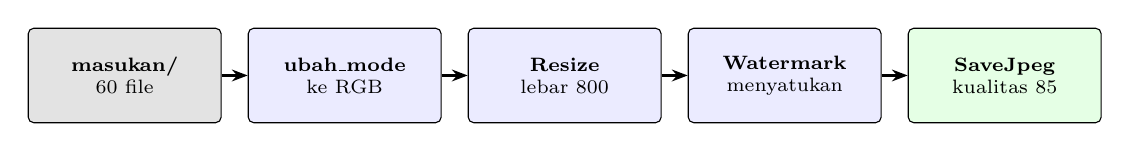
\begin{tikzpicture}[
    tahap/.style={draw, rounded corners=2pt, minimum width=2.45cm,
      minimum height=1.2cm, align=center, font=\scriptsize\bfseries},
    panah/.style={-{Stealth[length=2mm]}, thick}
  ]
    \node[tahap, fill=gray!22] (sumber) {masukan/\\
      {\scriptsize\mdseries 60 file}};
    \node[tahap, fill=blue!8, right=0.33cm of sumber] (mode) {ubah\_mode\\
      {\scriptsize\mdseries ke RGB}};
    \node[tahap, fill=blue!8, right=0.33cm of mode] (kecil) {Resize\\
      {\scriptsize\mdseries lebar 800}};
    \node[tahap, fill=blue!8, right=0.33cm of kecil] (tanda) {Watermark\\
      {\scriptsize\mdseries menyatukan}};
    \node[tahap, fill=green!10, right=0.33cm of tanda] (simpan) {SaveJpeg\\
      {\scriptsize\mdseries kualitas 85}};
    \draw[panah] (sumber) -- (mode);
    \draw[panah] (mode) -- (kecil);
    \draw[panah] (kecil) -- (tanda);
    \draw[panah] (tanda) -- (simpan);
  \end{tikzpicture}

  \vspace{10pt}
  {\small Setiap \textit{stage} hanya mengenal bentuk data yang lewat, bukan
  \textit{stage} di sebelahnya. \textit{Pipe} menyambung, dan tidak mengubah apa
  pun.}
\end{frame}

\begin{frame}[fragile]{{\Large Dua Bentuk \textit{Filter}}}
  \vspace{4pt}
\begin{lstlisting}[style=PythonStyle]
def ubah_mode(masukan):          # tanpa pengaturan
  for nama, gambar in masukan:
    yield nama, gambar.convert("RGB")

class Resize:                    # dengan pengaturan
  def __init__(self, lebar: int) -> None:
    self.lebar = lebar
  def __call__(self, masukan):
    for nama, gambar in masukan:
      yield nama, gambar.resize(...)
\end{lstlisting}
  \vspace{4pt}
  {\small \textit{Contract}-nya satu kalimat, yaitu satu \textit{iterable} masuk
  dan satu \textit{iterable} keluar. \textit{Pipe} memperlakukan keduanya dengan
  cara yang sama.}
\end{frame}

\begin{frame}{{\Large \textit{Class Diagram} \textit{Pipe} dan \textit{Filter}}}
  \vspace{2pt}
  \begin{center}
    % Lebarnya sedikit melebihi kolom teks lalu diletakkan di tengah dengan
    % makebox, sebab gambarnya lebar sehingga lebar itulah yang membatasi.
    \makebox[\textwidth][c]{%
      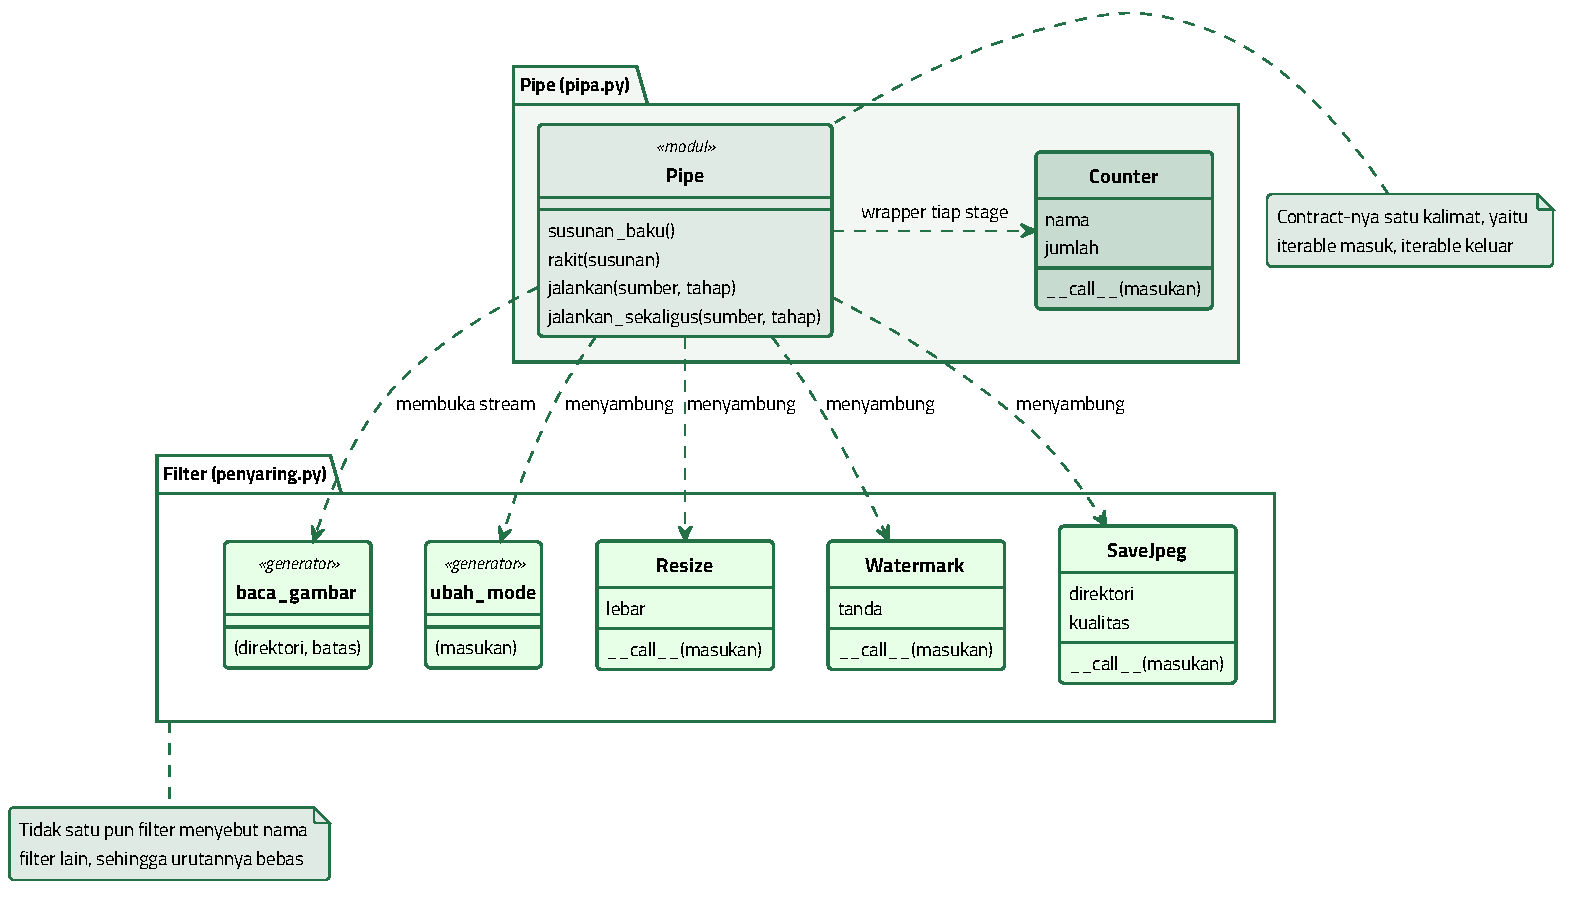
\includegraphics[width=1.12\textwidth, height=0.80\textheight,
        keepaspectratio]{kelas-pipa.pdf}}
  \end{center}
\end{frame}

\begin{frame}{{\Large Penjelasan \textit{Class Diagram}}}
  \vspace{10pt}
  \begin{itemize}\small
    \item Tidak ada satu pun panah antar \textit{filter}, sehingga urutannya
          bebas ditukar.
    \item \textit{Pipe} menyambung, dan dapat membungkus tiap \textit{stage}
          dengan \texttt{Counter}.
    \item \texttt{Counter} mencacah gambar yang lolos dari satu \textit{stage},
          sehingga jumlahnya dapat dilaporkan tanpa menyentuh isi
          \textit{filter}. Angka itulah yang dicatat pada Latihan 1.
    \item Dua \textit{filter} berupa fungsi generator, tiga lainnya berupa kelas
          yang dapat dipanggil.
    \item \texttt{periksa\_pipa.py} melaporkan nol penyebutan dari lima
          \textit{filter}.
  \end{itemize}

  \vspace{10pt}
  {\small Garis putus berkepala terbuka berarti \textit{dependency}, yaitu
  \textit{pipe} memanggil \textit{filter}, bukan sebaliknya.}
\end{frame}

\begin{frame}{{\Large Analogi: Lini Pengolahan Buah}}
  \vspace{10pt}
  \begin{itemize}\small
    \item Buah datang di atas \textit{conveyor belt}, lalu melewati meja
          pemilah.
    \item Jeruk diarahkan ke mesin pemeras, tomat diarahkan ke mesin
          penghalus.
    \item Setiap mesin hanya menangani buah yang datang kepadanya, dan tidak
          mengetahui proses di mesin yang lain.
    \item \textit{Conveyor belt}-nya sendiri tidak memproses buah apa pun.
  \end{itemize}

  \vspace{10pt}
  {\small Setiap mesin berperan sebagai \textit{filter}, sedangkan
  \textit{conveyor belt} berperan sebagai \textit{pipe}.}
\end{frame}

\begin{frame}{{\Large Menukar Dua \textit{Stage}}}
  \vspace{10pt}
  \begin{itemize}\small
    \item Yang ditukar \texttt{Resize} dan \texttt{Watermark}, sebab keduanya
          menerima dan menghasilkan bentuk data yang sama.
    \item Penukaran itu sah menurut \textit{contract}, sehingga \textit{pipe}
          menerimanya tanpa keberatan.
    \item Pertanyaannya, apakah penukaran yang sah selalu aman.
    \item Pengukurannya seratus putaran, sepuluh gambar tiap putaran, lalu
          seluruh \textit{file} keluarannya disidik dengan SHA-256.
  \end{itemize}

  \vspace{10pt}
  {\small Sidik dipakai untuk menjawab satu pertanyaan saja, yaitu apakah kedua
  urutan menghasilkan \textit{file} yang sama persis.}
\end{frame}

\begin{frame}{{\Large \textit{Stage Reordering}}}
  \vspace{6pt}
  {\small Kotaknya kuartil pertama sampai ketiga, garis tebal di dalamnya
  median, dan ujung kumisnya nilai terkecil serta terbesar.}

  \vspace{6pt}
  \centering
  \resizebox{0.92\textwidth}{!}{%
  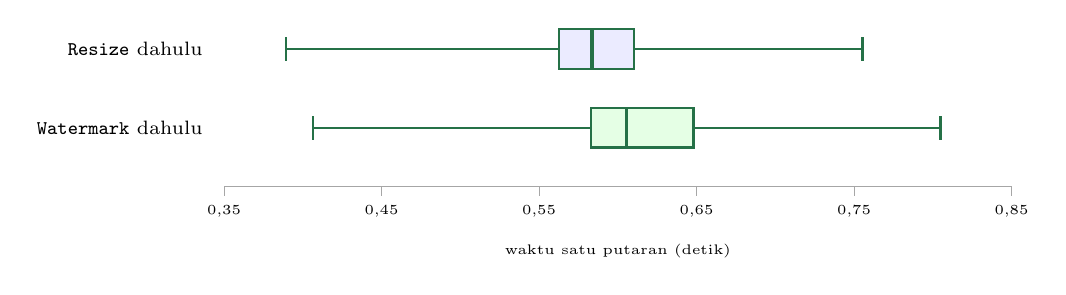
\begin{tikzpicture}[
      kotak/.style={draw=praditagreen, thick},
      sumbu/.style={draw=gray!70},
      label/.style={font=\scriptsize},
      kecil/.style={font=\tiny\mdseries}
    ]
      % Sumbu waktu, 1cm mewakili 0,05 detik mulai dari 0,35 detik.
      \draw[sumbu] (0,0) -- (10,0);
      \foreach \x/\teks in {0/0{,}35, 2/0{,}45, 4/0{,}55, 6/0{,}65, 8/0{,}75,
        10/0{,}85} {
        \draw[sumbu] (\x,0) -- (\x,-0.12);
        \node[kecil, below] at (\x,-0.12) {\teks};
      }
      \node[kecil, below] at (5,-0.6) {waktu satu putaran (detik)};
  
      % Urutan Resize dahulu: min 0,3893  Q1 0,5625  median 0,5835
      % Q3 0,6104  maks 0,7553
      \draw[kotak] (0.786,1.75) -- (4.25,1.75);
      \draw[kotak] (5.208,1.75) -- (8.106,1.75);
      \draw[kotak] (0.786,1.6) -- (0.786,1.9);
      \draw[kotak] (8.106,1.6) -- (8.106,1.9);
      \draw[kotak, fill=blue!8] (4.25,1.5) rectangle (5.208,2.0);
      \draw[kotak, very thick] (4.67,1.5) -- (4.67,2.0);
      \node[label, left] at (-0.15,1.75) {\texttt{Resize} dahulu};
  
      % Urutan Watermark dahulu: min 0,4065  Q1 0,5827  median 0,6054
      % Q3 0,6480  maks 0,8049
      \draw[kotak] (1.13,0.75) -- (4.654,0.75);
      \draw[kotak] (5.96,0.75) -- (9.098,0.75);
      \draw[kotak] (1.13,0.6) -- (1.13,0.9);
      \draw[kotak] (9.098,0.6) -- (9.098,0.9);
      \draw[kotak, fill=green!10] (4.654,0.5) rectangle (5.96,1.0);
      \draw[kotak, very thick] (5.108,0.5) -- (5.108,1.0);
      \node[label, left] at (-0.15,0.75) {\texttt{Watermark} dahulu};
    \end{tikzpicture}}

\end{frame}

\begin{frame}{{\Large Membaca Hasilnya}}
  \vspace{10pt}
  \begin{itemize}\small
    \item Kedua kotak hampir bertumpuk, sehingga satu putaran saja tidak
          memberi tahu urutan mana yang dijalankan.
    \item Arahnya tetap, yaitu \texttt{Resize} dahulu menang pada 88 dari 100
          putaran. Uji tanda menolak kebetulan dengan peluang di bawah dua per
          sepuluh pangkat lima belas.
    \item Besarnya kecil, yaitu 0,0219 detik, atau 3,8 persen dari median,
          sehingga tidak akan dirasakan pengguna.
    \item Yang pasti berbeda justru sidik \textit{file} keluarannya, yaitu
          \texttt{315e279c} melawan \texttt{28cdebf1}.
  \end{itemize}

  \vspace{10pt}
  {\small Urutan \textit{stage} di sini karena itu tidak layak dipilih
  berdasarkan waktu, melainkan berdasarkan hasilnya.}
\end{frame}

\begin{frame}{{\Large Apa Itu \textit{Fan-out} dan \textit{Merge}}}
  \vspace{10pt}
  \begin{itemize}\small
    \item \textit{Fan-out} berarti satu \textit{stream} digandakan menjadi
          beberapa \textit{stream} yang berjalan sendiri-sendiri, sehingga
          sumbernya cukup dibaca sekali.
    \item \textit{Merge} berarti beberapa \textit{stream} disatukan kembali
          menjadi satu.
    \item Pada contoh bab ini, satu foto sumber melayani tiga resolusi
          sekaligus, lalu laporan ketiganya disatukan.
  \end{itemize}

  \vspace{10pt}
  {\small Penggandaannya memakai \texttt{itertools.tee}, sedangkan
  penyatuannya memakai \texttt{itertools.chain}.}
\end{frame}


\begin{frame}{{\Large Jalur \textit{Fan-out} dan \textit{Merge}}}
  \vspace{10pt}
  \centering
  \resizebox{0.97\textwidth}{!}{%
  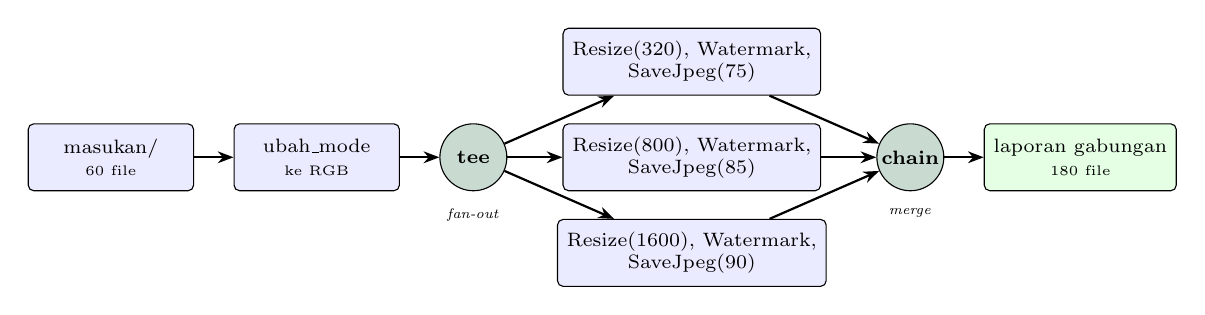
\begin{tikzpicture}[
      kotak/.style={draw, rounded corners=2pt, minimum width=2.1cm,
        minimum height=0.85cm, align=center, font=\scriptsize},
      hulu/.style={kotak, fill=blue!8},
      cabang/.style={kotak, fill=blue!8, minimum width=3.1cm},
      simpul/.style={draw, circle, fill=praditagreen!25, minimum size=0.85cm,
        inner sep=0pt, font=\scriptsize\bfseries},
      hasil/.style={kotak, fill=green!10, minimum width=2.4cm},
      panah/.style={-{Stealth[length=2mm]}, thick}
    ]
      \node[hulu] (sumber) {masukan/\\{\tiny\mdseries 60 file}};
      \node[hulu, right=0.5cm of sumber] (mode) {ubah\_mode\\{\tiny\mdseries ke RGB}};
      \node[simpul, right=0.5cm of mode] (tee) {tee};
  
      \node[cabang, right=0.7cm of tee] (sedang)
        {Resize(800), Watermark,\\SaveJpeg(85)};
      \node[cabang, above=0.35cm of sedang] (kecil)
        {Resize(320), Watermark,\\SaveJpeg(75)};
      \node[cabang, below=0.35cm of sedang] (besar)
        {Resize(1600), Watermark,\\SaveJpeg(90)};
  
      \node[simpul, right=0.7cm of sedang] (chain) {chain};
      \node[hasil, right=0.5cm of chain] (laporan)
        {laporan gabungan\\{\tiny\mdseries 180 file}};
  
      \draw[panah] (sumber) -- (mode);
      \draw[panah] (mode) -- (tee);
      \draw[panah] (tee) -- (kecil);
      \draw[panah] (tee) -- (sedang);
      \draw[panah] (tee) -- (besar);
      \draw[panah] (kecil) -- (chain);
      \draw[panah] (sedang) -- (chain);
      \draw[panah] (besar) -- (chain);
      \draw[panah] (chain) -- (laporan);
  
      \node[font=\tiny\mdseries, below=0.1cm of tee] {\textit{fan-out}};
      \node[font=\tiny\mdseries, below=0.1cm of chain] {\textit{merge}};
    \end{tikzpicture}}

  \vspace{10pt}
  \raggedright
  {\small Penyeragaman mode dikerjakan sekali di hulu, sebab hasilnya sama
  bagi ketiga cabang. Setiap cabang memakai lebar dan kualitas JPEG sendiri,
  lalu menulis ke direktorinya sendiri.}
\end{frame}

\begin{frame}{{\Large \textit{Fan-out} dan \textit{Merge}}}
  \vspace{4pt}
  \begin{center}
    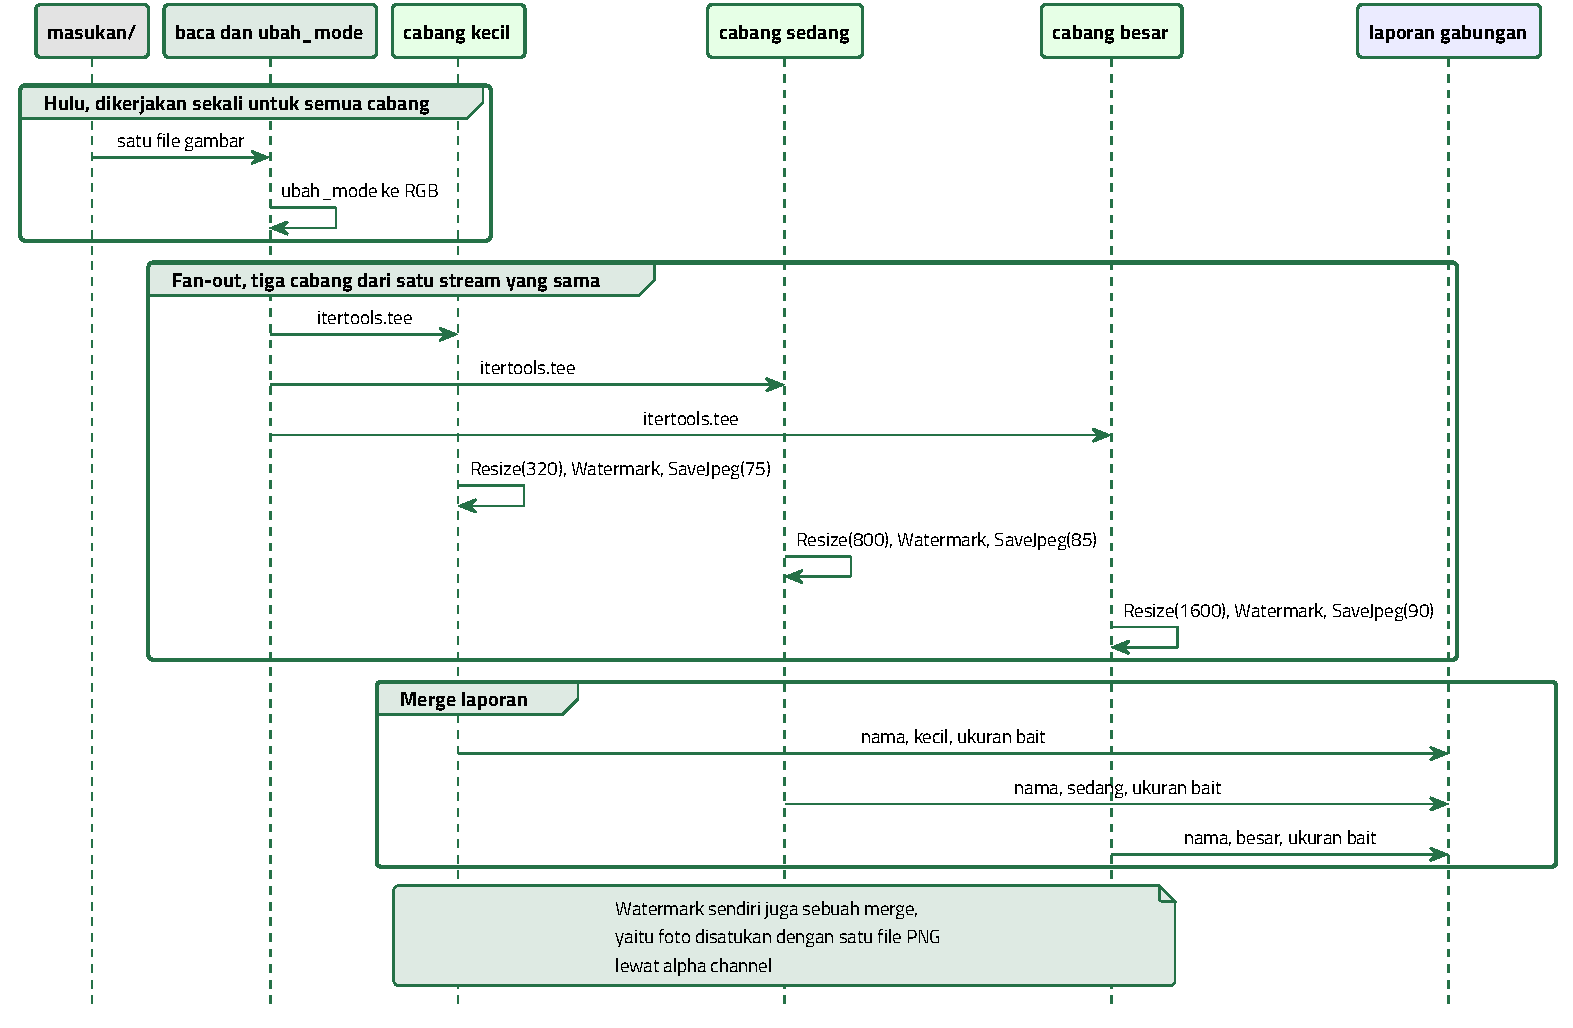
\includegraphics[width=\textwidth, height=0.74\textheight,
      keepaspectratio]{sekuens-percabangan.pdf}
  \end{center}
\end{frame}

\begin{frame}{{\Large Penjelasan \textit{Sequence Diagram}}}
  \vspace{10pt}
  \begin{itemize}\small
    \item Sumber dibaca sekali, lalu \textit{stream}-nya digandakan dengan
          \texttt{itertools.tee}.
    \item Penyeragaman mode dikerjakan di hulu, sebab hasilnya sama bagi ketiga
          cabang.
    \item Setiap cabang memakai lebar dan kualitas sendiri, lalu menulis ke
          direktori sendiri.
    \item Laporan ketiga cabang di-\textit{merge} kembali dengan
          \texttt{itertools.chain}.
  \end{itemize}

  \vspace{10pt}
  {\small \texttt{Watermark} sendiri juga sebuah \textit{merge}, yaitu foto
  disatukan dengan satu \textit{file} PNG lewat \textit{alpha channel}.}
\end{frame}

\begin{frame}{{\Large Tiga Resolusi dari Satu Pembacaan}}
  \vspace{6pt}
  {\small Keenam puluh foto sumber diunduh \texttt{unduh\_gambar.py} dari
  layanan Lorem Picsum memakai \textit{seed} tetap, yaitu \texttt{apl1} sampai
  \texttt{apl60} pada ukuran 1600 kali 1200 piksel, sehingga kumpulannya sama
  pada setiap mesin. Foto itu dibaca sekali, lalu \textit{stream}-nya digandakan
  menjadi tiga cabang dengan lebar dan kualitas JPEG sendiri. Angkanya dari
  keluaran \texttt{percabangan.py}.}

  \vspace{8pt}
  \centering
  \small
  \begin{tabularx}{0.9\textwidth}{|l|l|l|X|}
    \hline
    \textbf{Cabang} & \textbf{Lebar} & \textbf{Kualitas} & \textbf{Ukuran seluruhnya} \\
    \hline
    kecil & 320 & 75 & 723 KiB \\
    \hline
    sedang & 800 & 85 & 5.118 KiB \\
    \hline
    besar & 1600 & 90 & 15.697 KiB \\
    \hline
  \end{tabularx}

  \vspace{8pt}
  {\small Enam puluh \textit{file} sumber menghasilkan seratus delapan puluh
  \textit{file} keluaran, dan sumbernya cukup dibaca sekali.}
\end{frame}

\begin{frame}{{\Large Kasus: Belasan Ribu \textit{File}}}
  \vspace{8pt}
  \begin{enumerate}\small
    \item Pengolah foto membaca seluruh \textit{file} unggahan menjadi satu
          daftar, yaitu jalur \textit{batch}.
    \item Pada pengujian dengan tiga puluh \textit{file}, semuanya berjalan
          mulus.
    \item Pada hari pendaftaran, \textit{file} yang masuk mencapai belasan ribu.
    \item Proses berhenti karena kehabisan memori, dan tidak satu pun
          \textit{file} keluaran tertulis.
  \end{enumerate}

  \vspace{8pt}
  {\small \textit{Stage} penyimpanan memang belum sempat dimulai. Andai
  \textit{pipeline}-nya \textit{streaming}, \textit{file} pertama sudah tersimpan
  sejak detik pertama.}
\end{frame}

\begin{frame}{{\Large Hasil Pengukuran}}
  \vspace{6pt}
  {\small Seratus putaran, sepuluh gambar tiap putaran, dengan \textit{stage}
  yang sama persis pada kedua jalur. Yang diukur waktu sampai \textit{file}
  pertama selesai ditulis, lalu puncak \textit{Resident Set Size} (RSS), yaitu
  memori yang benar-benar dipegang proses menurut sistem operasi.}

  \vspace{8pt}
  \centering
  \small
  \begin{tabularx}{0.9\textwidth}{|X|l|l|}
    \hline
    \textbf{Yang diukur} & \textbf{\textit{Streaming}} & \textbf{\textit{Batch}} \\
    \hline
    Median \textit{file} pertama & 83,1 ms & 792,8 ms \\
    \hline
    Puncak RSS proses & 118,4 MiB & 576,8 MiB \\
    \hline
    Putaran dengan \textit{file} pertama lebih cepat & 100 dari 100 & 0 dari 100 \\
    \hline
  \end{tabularx}

  \vspace{8pt}
  {\small Puncak RSS diambil lewat \texttt{resource.getrusage} di dalam proses
  anak tersendiri, sebab angkanya tanda air tertinggi yang tidak pernah turun.}
\end{frame}

\begin{frame}{{\Large Ringkasan}}
  \vspace{10pt}
  \begin{itemize}\small
    \item \textit{Filter} tidak mengenal tetangganya, dan \textit{pipe}-lah yang
          menyambung mereka.
    \item \textit{Contract} yang seragam membuat \textit{stage} dapat ditambah,
          dibuang, atau ditukar tanpa menyunting \textit{stage} lain.
    \item Kebebasan itu berbatas pada bentuk data, dan penukaran yang sah pun
          belum tentu menghasilkan \textit{file} yang sama.
    \item \textit{Streaming} menyerahkan \textit{file} pertama 9,5 kali lebih
          cepat, dengan puncak RSS 118,4 MiB melawan 576,8 MiB.
  \end{itemize}

  \vspace{10pt}
  {\small Pesan utamanya, \textit{pipeline} memindahkan keputusan ke satu
  tempat, yaitu di luar \textit{filter}.}
\end{frame}

\begin{frame}[fragile]{{\Large Persiapan Latihan}}
  \vspace{5pt}
\begin{lstlisting}[language=bash]
bash sources/siapkan_venv.sh
source .venv/bin/activate
cd sources/chapter06
python unduh_gambar.py
# Gambar baru diunduh : 60
python buat_tanda_air.py
python pipa.py hitung
# Keluaran akhir: 60 file
\end{lstlisting}

  \vspace{6pt}
  {\small Tanpa jaringan, jalankan \texttt{python buat\_gambar.py} sebagai
  gantinya. Langkah lengkap, tabel contoh, dan lembar isian ada di modul Bab 6,
  yang menjadi rujukan utama latihan ini.}
\end{frame}

\begin{frame}[fragile]{{\Large Latihan 1: \textit{Filter Independence}}}
  \vspace{2pt}
  {\small Tujuan: membuktikan menambah \textit{stage} tidak menyentuh
  \textit{filter} lain.}

  \vspace{2pt}
\begin{lstlisting}[language=bash]
python periksa_pipa.py
# Filter ditemukan      : 5
# Filter menyebut filter: 0 {}
\end{lstlisting}

  \vspace{3pt}
  \begin{enumerate}\small
    \item Catat keempat angka yang dilaporkan.
    \item Tambahkan satu \textit{filter} baru yang memutar gambar, misalnya
          kelas \texttt{Rotate}, lalu sisipkan ke dalam susunan.
    \item Jalankan ulang, lalu catat berapa \textit{filter} lama yang perlu
          disunting.
  \end{enumerate}

  \vspace{3pt}
  {\small Pertanyaan: bagian mana yang membuat penambahan \textit{stage} tidak
  menyentuh \textit{filter} lain?}
\end{frame}

\begin{frame}[fragile]{{\Large Latihan 2: \textit{Stage Reordering}}}
  \vspace{2pt}
  {\small Tujuan: menguji apakah penukaran yang sah menurut \textit{contract}
  selalu aman.}

  \vspace{2pt}
\begin{lstlisting}[language=bash]
python uji_susun_ulang.py
# Putaran Resize lebih cepat : 88 dari 100
# File sama persis           : False
\end{lstlisting}

  \vspace{3pt}
  \begin{enumerate}\small
    \item Catat median, \textit{range}, pencacahan putaran, dan kedua sidiknya.
    \item Bandingkan ketajaman tanda air pada kedua direktori keluaran.
    \item Pindahkan \texttt{SaveJpeg} ke sebelum \texttt{Watermark}, lalu catat
          \textit{error}-nya.
  \end{enumerate}

  \vspace{3pt}
  {\small Pertanyaan: \textit{range}-nya 17 kali selisih median. Apakah
  selisih waktu itu layak disebut ada?}
\end{frame}

\begin{frame}[fragile]{{\Large Latihan 3: \textit{First Output Latency}}}
  \vspace{2pt}
  {\small Tujuan: mengukur harga menunggu seluruh data sebelum menulis.}

  \vspace{2pt}
\begin{lstlisting}[language=bash]
python ukur_aliran.py
# Puncak RSS streaming : 118.4 MiB
# Puncak RSS batch     : 576.8 MiB
\end{lstlisting}

  \vspace{3pt}
  \begin{enumerate}\small
    \item Catat kesembilan angka pada laporan akhirnya.
    \item Tunjukkan satu kata yang membedakan \texttt{jalankan} dari
          \texttt{jalankan\_sekaligus}.
    \item Turunkan \texttt{BATAS\_MEMORI} dari 60 menjadi 10, lalu catat
          perubahan puncak RSS-nya.
  \end{enumerate}

  \vspace{3pt}
  {\small Pertanyaan: mengapa selisih di sini layak disebut ada, sedangkan pada
  Latihan 2 tidak?}
\end{frame}

\end{document}
